% =====================================================================
%  Chapter 4 -- Stage 1: a smooth ramp in simulation
% =====================================================================
\chapter{Stage 1: A Smooth Ramp in Simulation}\label{ch:stage1}
\chapterlists

Before building anything, we asked in simulation: if $\RF$ is ramped smoothly through threshold, does
the circuit lag, and does the lag follow the $\sqrt{\lambda}$ law of \cref{sec:sqrt-law}?

\section{What we did}\label{sec:s1-setup}

With $\Ri=\SI{47}{\kilo\ohm}$ the ideal threshold lies at $\RF=\SI{94}{\kilo\ohm}$. The Wien network used
$R=\SI{1}{\kilo\ohm}$, $C=\SI{2}{\micro\farad}$ ($\wo=\SI{500}{\per\second}$); the simulated frequency,
\SI{78.8}{\hertz}, is within $1\%$ of $\wo/2\pi$. We ran
\begin{itemize}
  \item \textbf{upward} ramps $\RF(t)=\SI{93.5}{\kilo\ohm}+\lambda t$ from the quiet state, at 36 rates
        from \num{10} to \SI{10000}{\ohmpersec};
  \item \textbf{downward} ramps $\RF(t)=\SI{100}{\kilo\ohm}-\lambda t$ from full oscillation, at 28 rates
        from \num{40} to \SI{10000}{\ohmpersec},
\end{itemize}
and recorded the $\RF$ at which the oscillation switched on or off.

\section{What we saw}\label{sec:s1-results}

Nothing happens at the threshold (\cref{fig:s1-traces}). On the way up the output stays at noise level
well past \SI{94}{\kilo\ohm} and then rises abruptly; on the way down the oscillation survives well
below threshold before collapsing. The faster the ramp, the further the switching point moves from
threshold in both directions: Criterion~1, in simulation.

\begin{figure}[!htb]
  \centering
  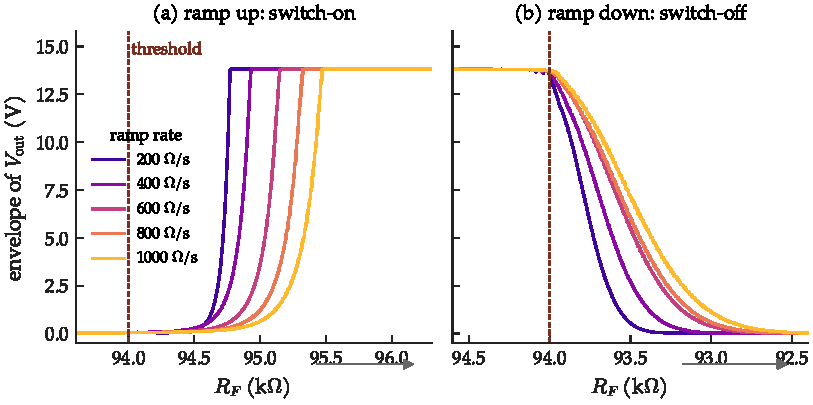
\includegraphics[width=\linewidth]{fig_s1_traces}
  \caption[Stage 1: response to smooth ramps]{Stage 1: output envelope against instantaneous $\RF$ for
  five ramp rates. (a)~Upward, from quiet. (b)~Downward, from full oscillation (axis reversed). Dashed:
  ideal threshold, \SI{94}{\kilo\ohm}.}
  \label{fig:s1-traces}
\end{figure}

The switching points (\cref{fig:s1-thresholds}a) follow \cref{eq:Ron,eq:Roff}:
\begin{align}
  \Ron  &= (\num{93924 \pm 13})\,\si{\ohm} + (\num{51.97 \pm 0.29})\sqrt{\lambda} , \label{eq:s1-on}\\
  \Roff &= (\num{94001.3 \pm 2.5})\,\si{\ohm} - (\num{29.62 \pm 0.05})\sqrt{\lambda} , \label{eq:s1-off}
\end{align}
with $\lambda$ in \si{\ohmpersec} and coefficients in \si{\ohm^{1/2}\,\second^{1/2}}.

\begin{figure}[!htb]
  \centering
  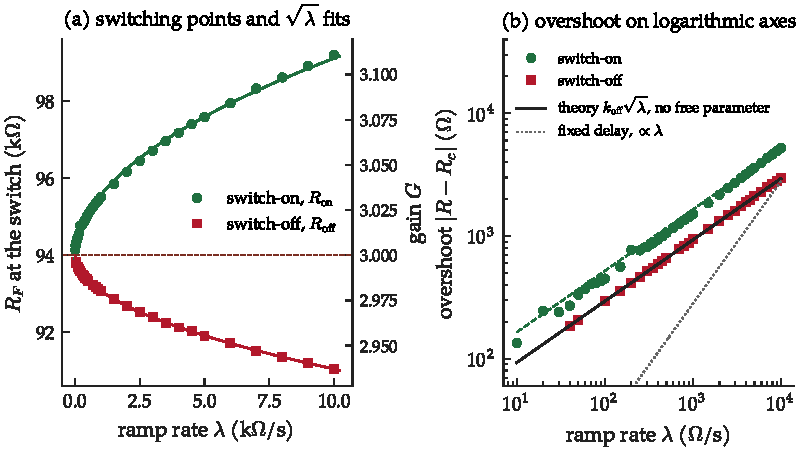
\includegraphics[width=\linewidth]{fig_s1_thresholds}
  \caption[Stage 1: switching points and the square-root law]{Stage 1: (a)~switching resistance against
  rate, with the fits of \cref{eq:s1-on,eq:s1-off}; (b)~overshoot on log axes. Switch-off points lie on the
  parameter-free prediction of \cref{eq:Roff} (black); a fixed delay would give slope one (dotted).}
  \label{fig:s1-thresholds}
\end{figure}

\paragraph{Threshold} Both intercepts match \SI{94}{\kilo\ohm} to better than $0.1\%$; the switch-off
intercept to within \SI{1.3}{\ohm}. The switch-on intercept lies \SI{76}{\ohm} below threshold, a
significant offset (see the next paragraph).

\paragraph{Exponent} With the exponent free, the fits give $0.499\pm0.003$ (off) and $0.546\pm0.005$ (on).
The switch-on exponent exceeds one half significantly. Together with the low intercept, this is
consistent with an effective noise floor that depends on the rate, which our fixed-$\delta$ derivation
ignores (\cref{sec:sqrt-law}); the switch-off law, which does not involve $\delta$, is the clean test.
A fixed delay, \cref{eq:fixed-delay}, fits more than twenty times worse (switch-off residuals
\SI{195}{\ohm} against \SI{7}{\ohm}).

\paragraph{Coefficient} For $\wo=\SI{500}{\per\second}$ and $\Ri=\SI{47}{\kilo\ohm}$, \cref{eq:Roff}
predicts
\begin{equation}
  k_{\mathrm{off}} = 2\sqrt{\frac{\ln 10\times\SI{47}{\kilo\ohm}}{\SI{500}{\per\second}}}
  = \SI{29.4}{\ohm^{1/2}\,\second^{1/2}} ,
  \label{eq:s1-koff-theory}
\end{equation}
within $1\%$ of the fitted $\num{29.62 \pm 0.05}$. Inverting \cref{eq:Ron}, the fitted $k_{\mathrm{on}}$
gives $\Lon=7.2$, an effective starting amplitude of about \SI{10}{\milli\volt}, larger than the
injected \SI{1}{\milli\volt}; how the two are related depends on the noise bandwidth, which we do not
model. The ratio
$k_{\mathrm{on}}/k_{\mathrm{off}}=1.75$ is the asymmetry of \cref{eq:k-ratio}.

\section{What this stage taught us}\label{sec:s1-learned}

\begin{learned}
\begin{itemize}[leftmargin=1.2em]
  \item \textbf{The circuit lags behind a moving threshold} in both directions (Criterion~1).
  \item \textbf{The lag grows as $\sqrt{\lambda}$}, exponent $0.499\pm0.003$, coefficient within $1\%$ of
        the parameter-free prediction (Criterion~2).
  \item \textbf{The effect is large}: more than \SI{5}{\kilo\ohm} at \SI{10}{\kilo\ohm\per\second}, many
        potentiometer steps.
\end{itemize}
\end{learned}

The effect was large enough for simple hardware. Next: would a real circuit, with real noise and a
resistance that moves in steps, behave the same way?
